%% 
% Preamble
%%
\documentclass[12pt]{article}

\usepackage{hyperref}
\usepackage{setspace}
\usepackage[tocbib,nosectionbib]{apacite}
\usepackage{amsmath}
%\usepackage[nomarkers, figuresonly]{endfloat} % All figures at end of document


\bibliographystyle{apacite}
    \renewcommand{\BOthers}[1]{\emph{et al.}.\hbox{}}
    \renewcommand{\BOthersPeriod}[1]{\emph{et al.}.\hbox{}}

\hypersetup{
    colorlinks = true,
    linkcolor = black,
    urlcolor = blue,
    citecolor = black,
    bookmarks = true}

\doublespacing
\usepackage[pdftex]{graphicx}
\usepackage{keyval}
\begin{document}

\setkeys{Gin}{width=\textwidth, resolution=72}

%%
% Title page
%%
\begin{titlepage}

\begin{center}

    \textbf{\LARGE Quantifying density cues in grouping displays}\\
    [3em]
    
\onehalfspacing{
    \large    
    Bart Machilsen, Johan Wagemans and Maarten Demeyer\\
    [2em]
    Laboratory of Experimental Psychology\\
    University of Leuven, Belgium\\
    [4em]
    \today
}
\end{center}

\vfill

\begin{flushleft}
\onehalfspacing{
    \textbf{All data and scripts}\\
    \href{https://github.com/mpjdem/densitycue}{https://github.com/mpjdem/densitycue}
}
\end{flushleft}


\begin{flushleft}
\onehalfspacing{
    \textbf{Corresponding author}\\
    Dr. Maarten Demeyer\\
    Tiensestraat 102\\
    3000 Leuven\\
    Belgium\\
    \href{mailto:maarten.demeyer@ppw.kuleuven.be}{maarten.demeyer@ppw.kuleuven.be}\\
    +32 16 326075\\
    [1.5em]
}
\end{flushleft}

\end{titlepage}

\newpage


%%
% Abstract
%%
\section*{Abstract}\label{section_abstract}
\thispagestyle{empty}

Perceptual grouping processes are typically studied using sparse displays of spatially separated elements. Unless the grouping cue of interest is a proximity cue, researchers will want to ascertain that such a cue is absent from the display. Various solutions to this problem have been employed in the literature; however, no validation of these methods exists. Here, we test a number of local density metrics both through their performance as constrained ideal observer models, and through a comparison with a large dataset of human detection trials. We conclude that for the selection of stimuli without a density cue, the \emph{Voronoi} density metric is preferable, especially if combined with a measurement of the distance to each element's nearest neighbor. We offer the entirety of the dataset as a benchmark for the evaluation of future, possibly improved, metrics. With regard to human processes of grouping by proximity, we found observers to be insensitive to target groupings that are more sparse than the surrounding distractor elements, and less sensitive to regularity cues in element positioning than to local clusterings of target elements. \\
[5em]
\textbf{Keywords}\\
perceptual grouping; contour integration; proximity; local density; ideal observer; Gabor displays; GERT

\newpage

%%
% Introduction
%%
\section{Introduction}\label{section_introduction}

The human visual system is capable of grouping spatially separated image features in the retinal input into coherent perceptual units. Empirical studies into the mechanisms underlying this process often employ stimuli composed of a large number of small image elements, that together elicit a global interpretation of the stimulus. For instance, in a typical contour integration stimulus \cite{Field93} a subset of collinearly aligned Gabor elements is perceived as a continuous path surrounded by randomly oriented distractor elements. However, since grouping by \emph{collinearity} is the subject of such a study, the placement of contour and background elements should be precisely controlled, in order to avoid an additional positional cue to the location of the embedded contour.\\

The problem is illustrated in \autoref{fig_density_illustration}. The left panel shows an array of oriented Gabor patches with an embedded open-ended contour. The percept of a smooth contour against a randomly oriented background appears to be due to the collinearity of neighboring Gabor patches. But, despite appearances, an additional cue besides the local alignment could contribute to the detection of the smooth contour here. In the right panel all local orientation information has been removed, and the path remains detectable through proximity or \emph{local density} cues to the location of the contour - either via explicit grouping mechanisms, or via a simple low-pass spatial frequency filter connecting nearby image elements. To eliminate the unwanted cue, the distribution of element spacings around contour and background elements needs to be controlled. In the literature, various methods have been proposed.\\

\begin{figure}[h]
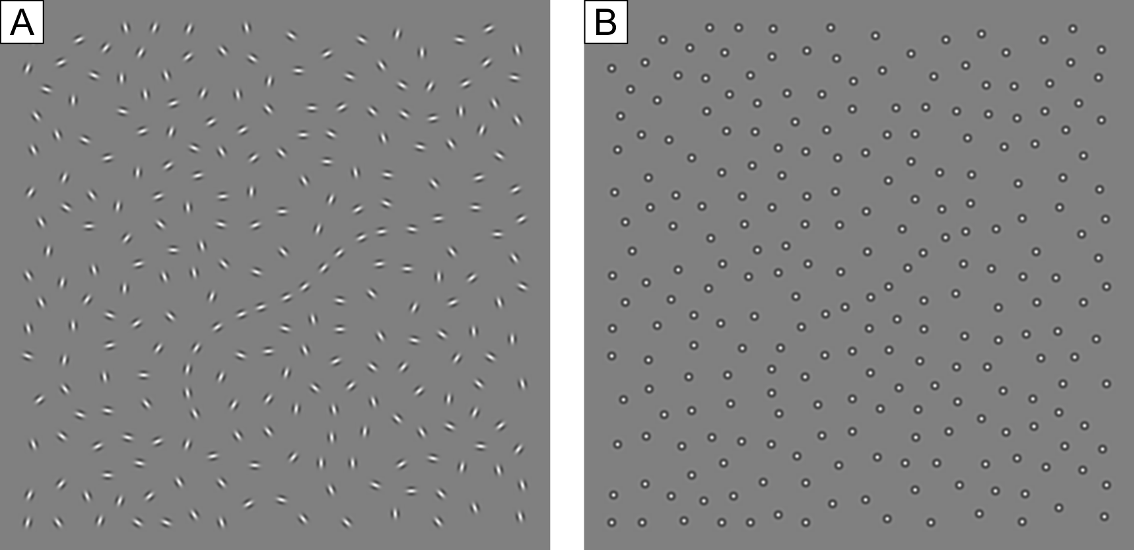
\includegraphics{Figures/FIG_density_illustration.png}
\caption{Local density cues in perceptual grouping displays. (A) The alignment of neighboring oriented Gabor elements gives rise to the percept of a smooth contour. (B) However, without orientation information the contour is still visible, because the neighboring element distances are distributed differently between contour and background elements.}
\label{fig_density_illustration}
\end{figure}

The \textbf{grid method} distributes all display elements evenly according to a latent grid. \citeA{Field93}, for instance, divided the stimulus display in squares corresponding to the desired eventual spacing between the contour elements. After the contour elements have been placed, background elements are inserted at a random location within each still empty grid cell. However, the use of such a grid does not by itself prevent systematic differences in the density profiles of contour and background elements \cite{Braun99}. Refinements of the grid method have been suggested to remove the residual density differences. For instance, \citeA{Nygard09} sampled the contour and background element locations from a shared distribution, and \citeA{Braun99} perturbs the initial grid configuration by a process simulating the diffusion of particles in a liquid.\\

The grid method of element placement has been criticized by \citeA{DakinBaruch09}, who argued that more uniform element densities can be obtained through pseudo-random placement of the elements. In this approach, contour elements are first placed as desired and background elements are then randomly added with a fixed minimum distance from previously placed elements \cite<e.g.,>{Kovacs94,Mijovic14,Sassi14,Watt08}. We have implemented this \textbf{minimal distance method} of element placement in our previously released toolbox GERT \cite<Grouping Elements Rendering Toolbox;>{Demeyer12}.\\

However, the element placement method is only the first step of local density control, since even the best random placement method might by chance result in a display containing a local density cue. This is where we found the literature to be lacking a consistent quantitative approach to the problem. Many researchers in the past have relied on visual inspection of the stimuli, or on visual inspection of density statistics computed from the displays \cite{Braun99}. This lack of a stringent control for local density cues is surprising given the well-known strength of proximity as a grouping cue \cite{ElderGoldberg02,KubovyWagemans95,Wertheimer23}, and the human sensitivity to local density variations \cite{Kovacs00,Tripathy99}.\\

One systematic approach can be found in the work of Kov{\'a}cs et al. \cite{Kovacs00, Kovacs93,Kovacs94,Kovacs99}, where the ratio D of the average background to average contour element distance is related to contour integration performance. These authors illustrate that density differences become irrelevant to human observers when D$<$1, that is, where the contour is more sparse in element density than the surrounding background elements.\\

In the GERT toolbox \cite{Demeyer12}, we instead implemented methods to completely eliminate the density cue, not only to human observers but also to ideal observers implemented in a computer algorithm. This generic framework offers quantitative decision criteria, applicable to various density metrics found in the literature. However, until now these metrics lacked validation. In the present study, we aimed to develop procedures for the quantitative evaluation of these and other local density metrics, and formulate recommendations for researchers in the field that are supported by empirical evidence. Three types of metrics are implemented in GERT.\\

\begin{figure}[h]
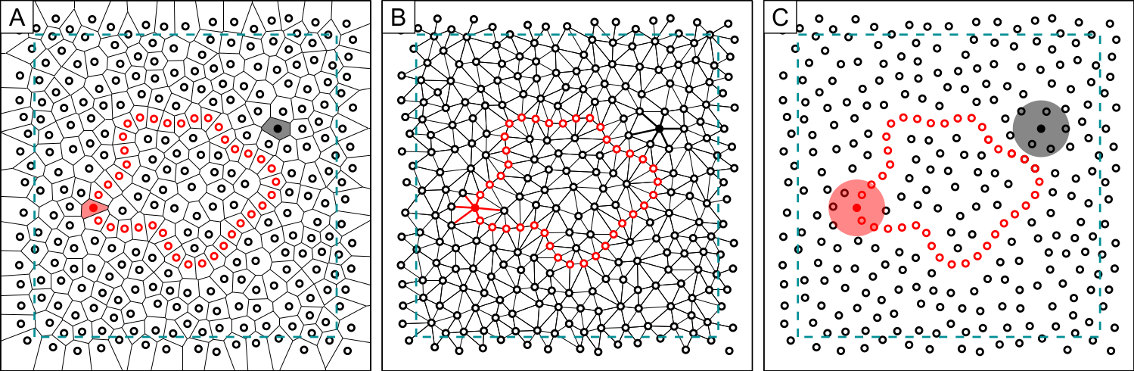
\includegraphics{Figures/FIG_metrics}
\caption{Schematic of the three types of local density metrics evaluated in this study. (A) \emph{Voronoi}. (B) \emph{AvgDist}. (C) \emph{RadCount}. See main text for more details.}
\label{fig_metrics}
\end{figure}

First, the \emph{Voronoi} metric, inspired by the methods used in \citeA{DakinBaruch09}, starts from a tessellation of the image space in polygon regions such that (a) each polygon contains only one element, and (b) all points within a polygon are closer to that element than to any other element in the display (\autoref{fig_metrics}A). The surface area of a polygon is then inversely related to the local density of the element contained within that polygon. To detect the presence of a density cue in the  display, we statistically compare the distribution of contour element local densities to those of background elements (see~\nameref{section_methods}).

Second, the \emph{AvgDist} metric computes the average distance from each element to its \emph{n} nearest neighbors. Below, we evaluate the performance of this metric for different values of \emph{n} (see \ref{subsection_methods_metrics}). In \autoref{fig_metrics}B the \emph{AvgDist} metric is illustrated for the `natural' neighbors of an element, as defined by a Delaunay triangulation of the image space \cite<neighboring Voronoi cells; see> {MathesFahle07}. This can be considered a parameter-free implementation of the \emph{AvgDist} metric.

Third, the \emph{RadCount} metric counts the number of neighboring elements within a circle of radius \emph{r} centered on each element of the display (\autoref{fig_metrics}C). This number, normalized by the area of the circle, is then taken as the local density measurement of each element. GERT (1.3+) also implements a parameter-free variant of the \emph{RadCount} metric, where a range of radii is tested \cite{Braun99}. The sum of the absolute mean differences between contour and background, across all radii, is then used as the local density measure (see \ref{subsection_methods_metrics}).\\

In the present study, we compared these three metrics of local density cues, and evaluated both (1) the performance of \emph{constrained ideal observer models} implementing each metric in detecting the presence of the physical density cue, and (2) how these ideal observer results relate to human performance in detecting embedded contours on the basis of a local density cue. For metrics with a free parameter, \emph{AvgDist} and \emph{RadCount}, we in addition tested a range of plausible parameter values.\\

The comparison to human detection performance requires the collection of empirical data on local density perception. A two-interval forced-choice (2-IFC) contour detection task was run, explicitly requiring the use of positional information to discriminate between a target (with embedded contour) and a distractor (with randomly placed background elements only). Orientation-less circular Gabor elements were used as display elements. These stimuli eliminated all interactions with element orientation, and yet maintained a high degree of similarity to previous studies on contour integration. We regard grouping by local density in such \emph{circular} Gabor fields as a liberal estimate of the influence of positional information on contour integration in more conventional arrays of \emph{oriented} Gabors.

To evaluate the generalizability of a metric's performance across different display types, we furthermore created a 2x2x2 design matrix of Sparse versus Dense display density, Open versus Closed contours, and Equidistant versus Randomly placed contour elements.
Since the constrained ideal observer models of each metric performed the same 2-IFC task, with the same stimuli, a direct comparison of physical cue detection to human performance was possible.\\ 

Two experiments were run. In Experiment 1, full psychometric curves were measured for a range of contour element spacings, from far more dense than the background element spacing to around the equality point; note however that this equality point is in practice not straightforward to establish, see \citeA{Demeyer12}. In Experiment 2, we followed up on the suggestion in the literature that, without orientation information, human observers are unable to detect contours with an element density that is sparser than the surrounding background \cite{Kovacs99}. If only the human detectability, rather than the presence of a cue to ideal observers, is of interest to the researcher, such a display selection criterion might indeed be useful. To verify this claim through methods comparable to those applied to the results of Experiment 1, we here explicitly required subjects to detect contours at a single sparse contour spacing level.


%%
% Methods
%%
\section{Methods}\label{section_methods}

\subsection{Participants}\label{subsection_methods_participants}
In Experiment 1, eight subjects (four male, four female, mean age: 24y, age range: 18-32y) with normal or corrected-to-normal sight participated in the experiment. Five participants were naive as to the purpose of the study. They received a monetary reward for their participation. Among the non-naive participants were the authors BM and MD. Written informed consent was obtained from each naive participant. Ethical approval in line with the Declaration of Helsinki was obtained from the ethical committee at the University of Leuven.

In Experiment 2, six subjects participated under the same conditions. Except for two female participants, one naive and one non-naive, none of them authors, these subjects were the same as in Experiment 1.


\subsection{Apparatus}\label{subsection_methods_apparatus}

Both experiments were run in a dimly lit room on a 22\verb+"+ CRT monitor (Iiyama Vision Master Pro 514; diameter of viewable screen size: 51 cm). The refresh rate was 85 Hz, and the spatial resolution of the screen 1024 $\times$ 768 pixels. At a viewing distance of 100 cm the apparent stimulus size was 11.6 degrees of visual angle. Stimulus presentation was controlled by PsychToolbox 3.0.9 \cite{Brainard97} using Matlab R2009b (7.9; The MathWorks) on a Dell Precision T3400 workstation with an NVIDIA Quadro FX570 graphics card.

To linearize stimulus luminances, we measured the screen luminance once before data collection using a Konica Minolta CS-100 handheld luminance meter. We measured the screen luminance (in cd/m$^2$) of 15 linearly spaced grayscale levels from 0 to 1. A power function with intercept 0 was fitted to these measurements, and the inverse of this function was used to transform all stimuli during stimulus presentation. The full luminance range of the monitor (with a maximum luminance of 48.9 cd/m$^2$) remained available.

As response keys, the subjects could use two analog buttons of the breaker type, connected to the parallel port of the computer.

\subsection{Stimuli and conditions}\label{subsection_methods_stimuli}

All stimuli were created before the start of the experiment using GERT v1.11 (\citeA{Demeyer12}; \href{http://www.gestaltrevision.be/gert}{www.gestaltrevision.be/gert}) under Matlab 7.9 and Windows XP SP3.\\

The stimulus displays consisted of arrays of circular Gabor patches on an isoluminant mid-gray background luminance of 0.5 (see example stimulus in \autoref{fig_density_illustration}B). The image size was 512 $\times$ 512 pixels. A circular Gabor element was defined as the product of a radial sinusoidal grating and an isotropic 2-D Gaussian. The luminance $L$ at each pixel $p$ is given by:
\begin{center}$L _p = \cos(\phi + \omega \lVert \mathbf{p} \rVert)\exp{(\frac{-\lVert \mathbf{p} \rVert ^{2}}{2\sigma^{2}})}$.\\\end{center}

$\lVert \mathbf{p} \rVert$  denotes the Euclidean distance from the center of the patch to the pixel location. The radial sinusoidal grating had a phase $\phi$ of 0 and a frequency $\omega$ of 0.1 cycles per pixel. The Gaussian envelope had a standard deviation $\sigma$ of 2.5 pixels in both dimensions. All circular Gabor elements were identical, with a maximal luminance of 1 and a minimal luminance of 0.387. Individual element patches were rendered on a canvas of 21 $\times$ 21 pixels, that was then pasted into the overall image.

The contour elements in a target display were positioned on an underlying radial frequency pattern (RFP) contour \cite{WilkinsonEtAl98}. An RFP contour is a smooth multi-lobed contour, here generated by adding (in a polar coordinate system) four sine wave modulations to a circle with a radius of 100 pixels. The frequencies of the component sine waves were randomly drawn, without replacement, from the set $\{2,3,4,5,6\}$. Each sine wave had a random phase offset and a random amplitude between 7.5 and 12.5 pixels. The center of the RFP polar coordinate system was aligned to the center of the stimulus display. The main difference between RFP contours and the snake stimuli typically used in pathfinder displays is that RFP contours are continuous, whereas snakes are composed of a discrete set of connected line segments. A continuous contour definition allows the positioning of elements at any location along the contour.\\

\begin{figure}[ht]
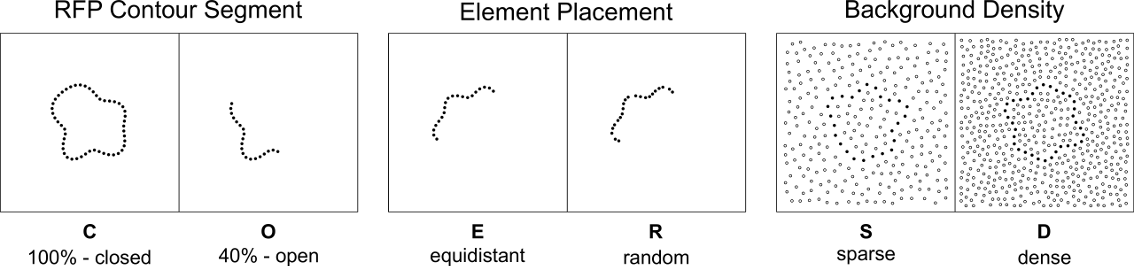
\includegraphics{Figures/FIG_conditions.png}
\caption{Diagram of stimulus conditions. Eight stimulus conditions were created by cross-combining three stimulus features: (1) The embedded RFP contour (radial frequency pattern) could be closed or open. (2) Contour elements could be placed at equidistant or at random locations along the contour. (3) The overall background spacing between elements could be large (sparse displays) or small (dense displays).}
\label{fig_conditions}
\end{figure}

To assess the generalizability of our results across different  display types, we cross-combined three stimulus characteristics: open \emph{vs.} closed contour, equidistant \emph{vs.} random placement of elements on the contour, and sparsely \emph{vs.} densely populated displays. (1) For closed contours, elements were positioned along the entire RFP contour definition. For open contours, only a random 40\% segment of the RFP contour definition was used. (2) Elements could be positioned at equally spaced locations along the contour (equidistant condition), or at random locations. In both cases a minimum distance between the contour elements was specified (see below). (3) Finally, we embedded the contours in arrays with relatively few background elements (sparse condition) or with many background elements (dense condition). The spacing between contour elements depended on the density of the background, to maintain the same difficulty level for the human observers (see below). Background element placement continued until no more elements could be added without violating the minimum distance requirement. This minimum distance was also respected  with regard to the display border. 

Two example target stimuli are shown in \autoref{fig_conditions_rendered}A and \autoref{fig_conditions_rendered}B.\\

Distractor stimuli were created by filling an empty display, using the same background density parameters as in the corresponding target displays (see \autoref{fig_conditions_rendered}C). For each of the eight display type conditions and each of the eight contour spacing conditions, 50 different target stimuli were generated. For each contour spacing condition, 50 different distractor stimuli were generated.\\

\emph{Experiment 1.} For each display type the strength of the local density cue was systematically varied in eight discrete steps, by manipulating the distance between adjacent contour elements. The optimal range of minimum distances was determined in a pilot experiment with three non-naive participants (including the authors BM and MD), aiming at a performance of 100\% correct for the smallest average spacing between contour elements, and 50\% correct (chance-level) for the largest spacing. Naturally, the minimum distances are different for sparse and dense displays.

For Sparse displays, the minimum Euclidean distance between a background element and any other element was 23.5 pixels. Equidistant placement of contour elements in Sparse displays respected a distance \emph{along the contour} of 19 to 27.5 pixels, in eight linearly spaced steps. In the case of Random element placement, an \emph{Euclidean} minimum distance from 16 to 25 pixels was imposed, again in eight linearly spaced steps. Dense displays used a minimum background element distance of 16.5 pixels, and contour distances of 11 to 17.5 pixels (Random) and 14 to 20 pixels (Equidistant).\\

\emph{Experiment 2.} Only a single level of contour spacing was used in Experiment 2. The same eight display type conditions were tested. To determine a suitable value of contour spacing we aimed at a performance of 75\% correct under the assumption that only the magnitude of the density cue, and not its direction, determines task performance. Under this assumption, a performance of about 75\% correct can be expected when adding half the interval width of spacing values used in Experiment 1 to the highest spacing value used in Experiment 1. For Sparse displays this resulted in a distance between contour elements of 31.75 pixels in the Equidistant conditions, and 29.5 pixels in the Random conditions; for Dense displays this resulted in 23 pixels in the Equidistant conditions, and 20.75 pixels in the Random conditions.

\begin{figure}[h]
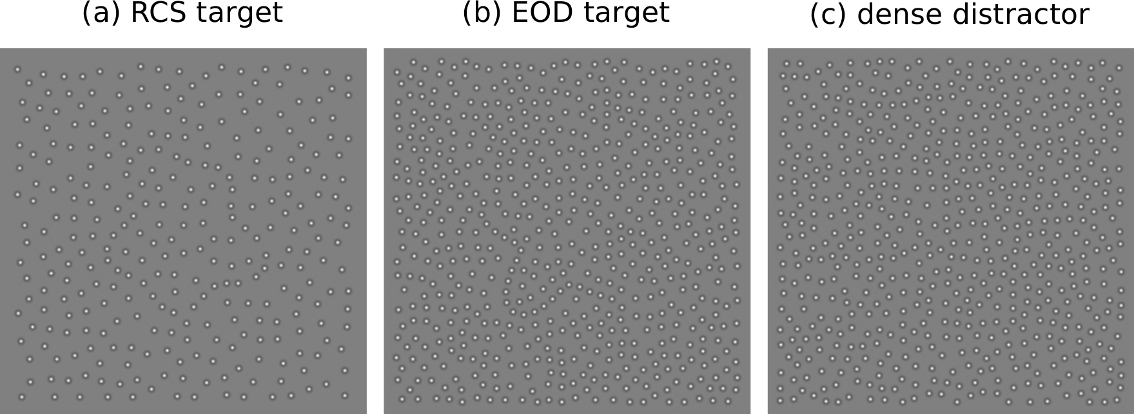
\includegraphics{Figures/FIG_conditions_rendered.png}
\caption{Example stimuli. Only two of the eight different target conditions are illustrated. (A) An example RCS target display with \textbf{R}andom element placement on a \textbf{C}losed contour in a \textbf{S}parse display. In this example the minimum Euclidean density between contour elements is 19 pixels. (B) An example EOD target display with \textbf{E}quidistant element placement on an \textbf{O}pen contour in a \textbf{D}ense display. In this example the distance between consecutive elements along the contour is 14.86 pixels. (C) An example dense distractor display with no embedded contour.}
\label{fig_conditions_rendered}
\end{figure}

\subsection{Task and procedure}\label{subsection_methods_procedure}
\subsubsection{Experiment 1}
A 2-IFC task was run to estimate human sensitivity to local density cues under different stimulus conditions. Participants were asked to indicate which of two sequentially presented displays contained a contour, as defined by local density differences between contour and background elements. All observers were first run through a practice session before starting the actual experiment. During the practice trials, the eight display types were intermixed. The difficulty level gradually increased. In the first two blocks of trials, only the two easiest contour spacing levels were shown. The next two blocks contained the four easiest conditions. In the final two blocks of practice trials all contour spacing levels were used. The main experiment started after completing 240 trials of the practice session.\\

\begin{figure}[h]
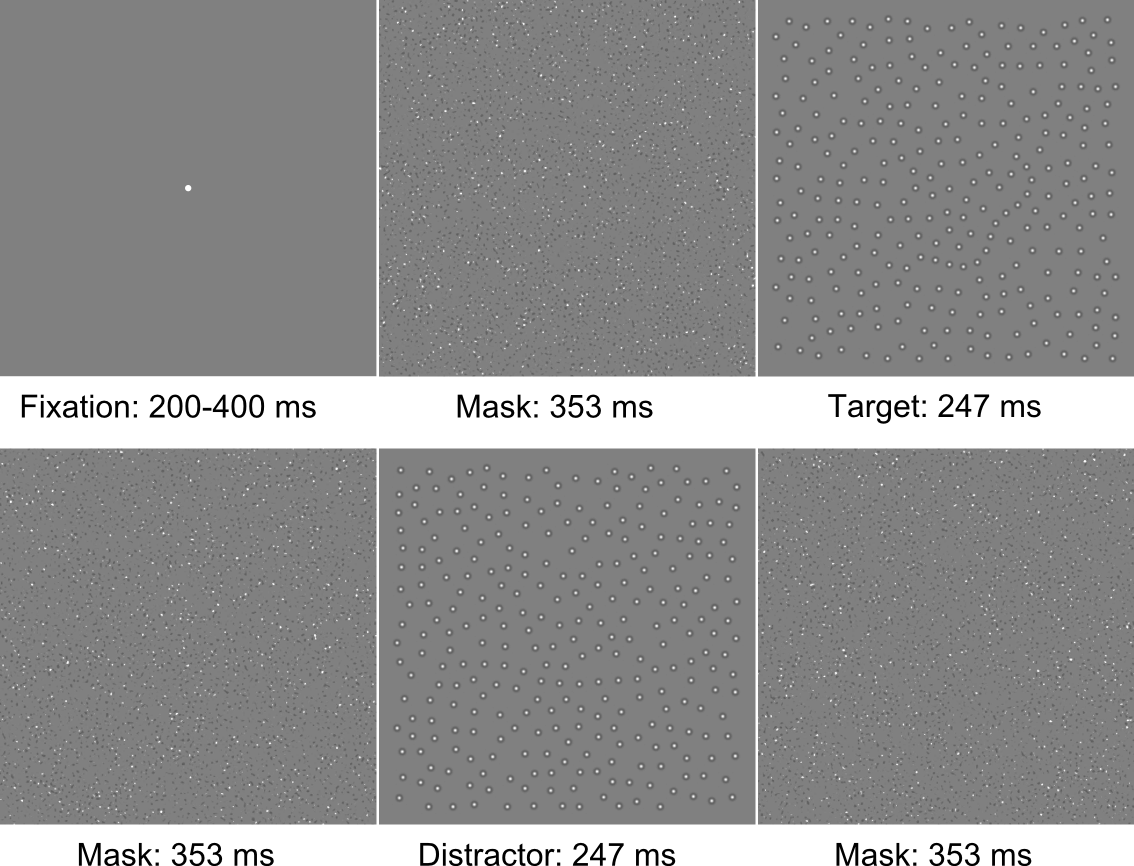
\includegraphics{Figures/FIG_trial.png}
\caption{Time-course of a 2-IFC trial. The order of target and distractor intervals was random. Target and distractors were both forward and backward masked. The target condition in this example is EOS: equidistant placement of elements on an open contour in a sparse display.}
\label{fig_trial}
\end{figure}

In the main experiment we used the method of constant stimuli, with eight levels of contour spacing, to measure psychometric curves for all eight display type conditions. Target and distractor displays always used the same background element density. Each of these 64 conditions was presented in 100 trials each. The stimulus conditions and levels of contour spacing were fully randomized on a trial-by-trial basis. Stimuli were presented in blocks of 100 trials. Participants were allowed to pause after each block of trials. A single session of eight blocks lasted around one hour. The main experiment was completed after eight of these sessions (6400 trials per participant).\\

\autoref{fig_trial} illustrates the time course of a single trial. After preloading the stimuli (+-200 ms) a white fixation dot was presented for a variable duration between 200 and 400 ms. Participants were instructed to maintain fixation throughout the experiment. Target and distractor displays were presented for 247 ms and were forward and backward masked with three different mask displays, each presented for 353 ms. Masks were created by phase-scrambling distractor images of corresponding background density according to a von Mises distribution. The order of the target and distractor displays was randomly determined on each trial. Two very brief sine wave sounds accompanied the target and distractor intervals to help participants with pacing. At the end of each trial, the screen turned to mid-gray and participants indicated through a button press the perceived target interval. The left button corresponded to the first interval, the right button corresponded to the second interval. Auditory feedback was provided after each trial. In case of a late response ($>$1000 ms), multiple simultaneous button presses or a wrong response, a lower frequency sine wave sound was played. In case of a correct response, a higher frequency sound was played. The next trial started automatically after a response was received, or after a time-out period of 1000 ms.

\subsubsection{Experiment 2}
No practice session was run prior to Experiment 2, since subjects were already familiar with the general task. However, we did add the explicit instruction to detect embedded contours that were \emph{less} dense than the background, and warned subjects that this could be difficult. One hundred trials were run for each display type, resulting in a total of 800 trials, collected over the course of a single one-hour session.


\subsection{Psychometric functions}\label{subsection_methods_curves}

In Experiment 1, we obtained for each participant and each display type 800 responses, 100 for each level of contour spacing. Trials without a valid response (late response or simultaneous keypresses) were first excluded from the dataset ($<$0.7\%). A logistic function was then fit to the 800 binary responses (correct/incorrect) using Matlab's \emph{glmfit} with a modified binomial link function, accommodating a lower asymptote of 50\% correct. In cases of (quasi-) complete separation of data points the fits were optimized by minimizing the negative log-likelihood using Matlab's \emph{fminsearch} function. From the resulting intercept $c$ and slope $s$ of the logistic fit, we determined for each stimulus condition and for each participant the 75\%-threshold as $-c/s$.

In Experiment 2, only one level of contour element spacing was measured, and no psychometric curve could therefore be fit.


\subsection{Local density metrics}\label{subsection_methods_metrics}

All local density computations (see \autoref{fig_metrics}) were done using GERT version 1.3 \cite{Demeyer12}. \\

The \emph{Voronoi} metric is parameter-free. The \emph{AvgDist} metric was run parameter-free, using the natural neighbors of each element, as well as with a fixed number of neighbors. The values used were 1, 2, 3, 4 and 5. For the \emph{RadCount} metric we used fixed radius parameters ranging from 1.25 to 2.25 times the minimal background element distance, in linearly spaced steps of 0.25. In addition the parameter-free variant (\emph{RadCountFull}) was run using 20 different radii, linearly spaced between 1 and 2 times the minimal background element distance.

We did not compute local density values for elements closer to the display border than twice the minimum distance between background elements (blue dotted line in \autoref{fig_metrics}), because these elements naturally have fewer neighbors, and hence a smaller local density value.\\

For each local density metric and each display we obtained a distribution of local density values for the elements belonging to the contour and for the elements belonging to the background. From this, we computed for each display the overall difference in local density between contour and background by simply subtracting the means of the two distributions. The size of this difference is indicative for the presence of a local density cue. To evaluate whether an observed difference is significant we ran a Monte Carlo permutation test. We randomly reassigned the element labels (\emph{contour} vs. \emph{background}) 1,000 times. For each resampling, we again computed the mean difference between the randomly assigned contour-labeled and background-labeled elements. We then compared the true observed difference against this distribution of differences obtained through randomly permuting the element labels. This allows the computation of the proportion \emph{p} of resampled differences that are more extreme than the observed difference. A display with a \emph{p} of 0 indicates that the contour is more dense than the background to a degree not seen in any of the 1,000 resamplings. A \emph{p} of 1 similarly indicates that the background is more dense. For a display devoid of any local density cue, given a specific metric, \emph{p} equals .5.\\

Computing the \emph{p} for distractor displays is slightly more complicated because these displays do not have any contour elements. To allow for a comparison with the target displays, we labeled a subset of background elements in the distractor displays as `pseudo-contour' elements. This was done through computing which elements in the distractor display were closest in Euclidean distance to the contour definition latent to the target display of the trial.


\subsection{Ideal observer analysis}\label{subsection_methods_io}

In contrast with the human observers, the ideal observers we used were \emph{informed} ideal observers: They know which elements are the contour and the background elements. This was done to prevent a circularity in the application of these results to contour integration research. Not informing the ideal observers of the contour location would imply the implementation of a pathfinder algorithm, while the goal of contour integration research is often exactly the discovery of such an algorithm in the visual system. Moreover, providing this information could only introduce a conservative bias to display selection, where ideal observer metrics detect cues more easily than humans would. 

At the same time however, these informed ideal observers are also \emph{constrained} ideal observers, since each one of them uses only one specific local density metric with a given parameter setting.\\

All ideal observers executed the same task, in the same stimulus order, as the human participants did: To decide which of two displays contained the target. On each trial, the ideal observer selected the display with the most extreme \emph{p} (i.e., highest $|p - .50|$) as its response, i.e. the suspected target display. We acquired for each trial in the experiment the binary responses (correct/incorrect) of each ideal observer. In Experiment 1, psychometric functions were fitted to these data, following the same procedure applied to the human responses. At the highest levels of contour spacing however, some ideal observers correctly identified the target display based on a density difference in the opposite direction; that is, with contour elements judged as being less dense than background elements. We suspected from the literature \cite<e.g.,>{Kovacs00}, and will confirm in Experiment 2, that subjects are likely to perform at chance for such contours. Therefore, to ensure a similar monotonic decrease in performance with increasing contour spacing for the ideal observer models, data points where according to the metric the average contour density was \emph{more} sparse than the background density were fixed at 0.50 (chance level) when fitting the psychometric function. Of course, this introduces a deviation from the 'ideal' performance of these observers. We will however assess performance on this side of the contour density continuum separately in Experiment 2.\\

The ideal observer responses were used for two separate purposes. First, we compared the performance between all ideal observers to find the one that is most sensitive to the physically present local density difference. Second, we compared the performance of each ideal observer to the performance of our human observers. This allowed us to determine what kind of local density information human observers can use in practice. Details of the comparison methods are given in the \nameref{section_results} section.\\


\subsection{Statistical testing}\label{subsection_methods_stats}

The constrained ideal observers yielded for each stimulus condition a single point-estimate for the 75\%-threshold. A statistical comparison between the thresholds of the ideal observers, however, requires an estimate of the variability around the point-estimates. Moreover, peculiarities of the specific randomly selected target and distractor displays used in the experiment may result in biased point-estimates for the thresholds. To surpass these limitations, we recomputed the 75\%-thresholds in a resampling procedure. We resampled with replacement the performances of the 50 stimulus sets used for each condition, then re-averaged them into a condition performance, and re-computed the thresholds using psychometric curve fitting. The same trial resampling order was re-used across all metrics to be compared. After repeating this procedure 1,000 times, the standard error of each 75\%-threshold could be computed. These standard errors were then used to statistically evaluate differences between local density metrics. The same general procedure was followed in the other statistical analyses involving the ideal observer models.

%% 
% Results Experiment 1
%%
\section{Results}\label{section_results}
\subsection{Human obervers: Detection}\label{subsection_results_detect_human}
\subsubsection{Experiment 1}

\begin{figure}[h!t]
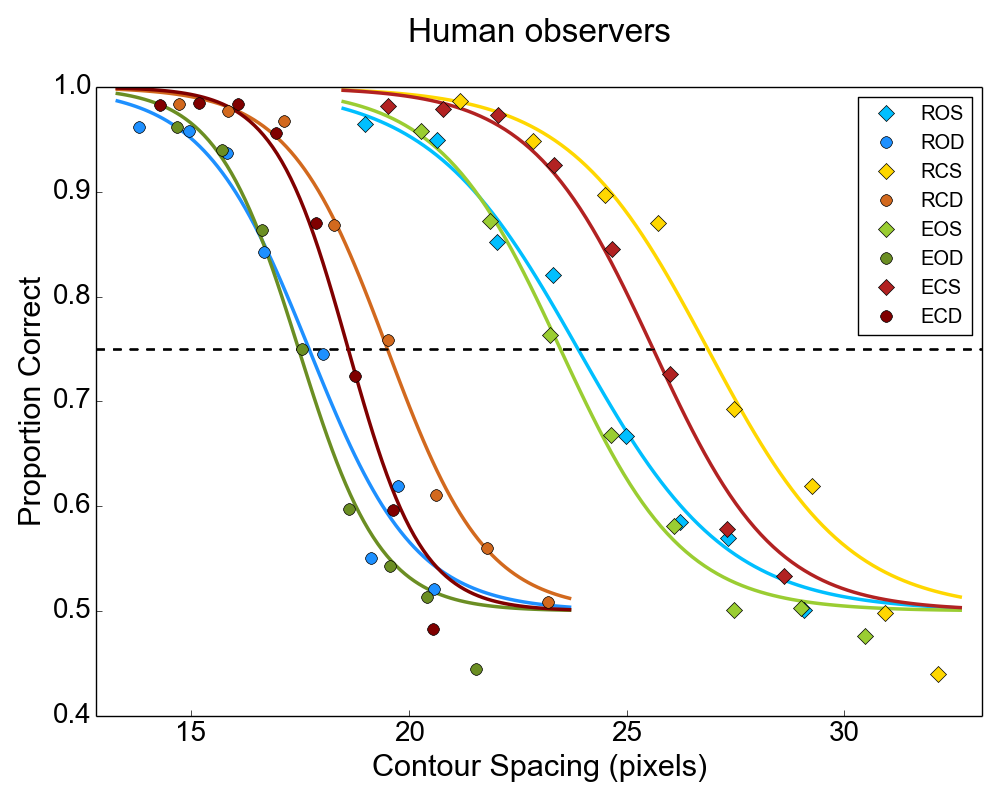
\includegraphics{Figures/FIG_detect_data_exp1.png}
\caption{Human performance in Experiment 1. The markers denote the average proportion of correct responses across observers, for the eight stimulus conditions (see legend) and the eight levels of contour spacing. The logistic fits to these data points are shown (see main text). The dotted horizontal line represents the 75\%-threshold. The condition labels correspond to \autoref{fig_conditions}: R = random; E = equidistant; O = open; C = closed; S = sparse; D = dense.}
\label{fig_human_exp1}
\end{figure}

\autoref{fig_human_exp1} shows the average performance across all participants for the eight stimulus conditions, and the corresponding logistic fits. Note that we computed the contour  spacing values on the X-axis as the actual average Euclidean distance between subsequent contour elements, instead of using the (sometimes incompatible) theoretical stimulus parameters. This explains why the different conditions have different X-axis values, although all cover the full 50\% to 100\% performance range.

We did not run statistical tests on these data. The different stimulus conditions were not designed to allow a direct comparison between them. They were only included to assess the generalizability of our findings to a wide range of grouping displays. In \autoref{subsection_results_predict} we will formally compare the human data and the ideal observer models. Here, however, we only offer a qualitative description of the human data.\\

As expected, performance in the 2-IFC task decreased with increasing distance between contour elements. Closed contours were systematically better detected than open contours, confirming the closure superiority reported by \citeA{Pettet98}. Is is however important to note that open and closed contour stimuli differed in more than just contour closure (e.g., number of contour elements; \citeA<see also>{Tversky04}). In addition, random placement of contour elements led to better performance than equidistant placement of contour elements. All results were qualitatively identical in sparse and dense displays.

\subsubsection{Experiment 2}

\begin{figure}[h!t]
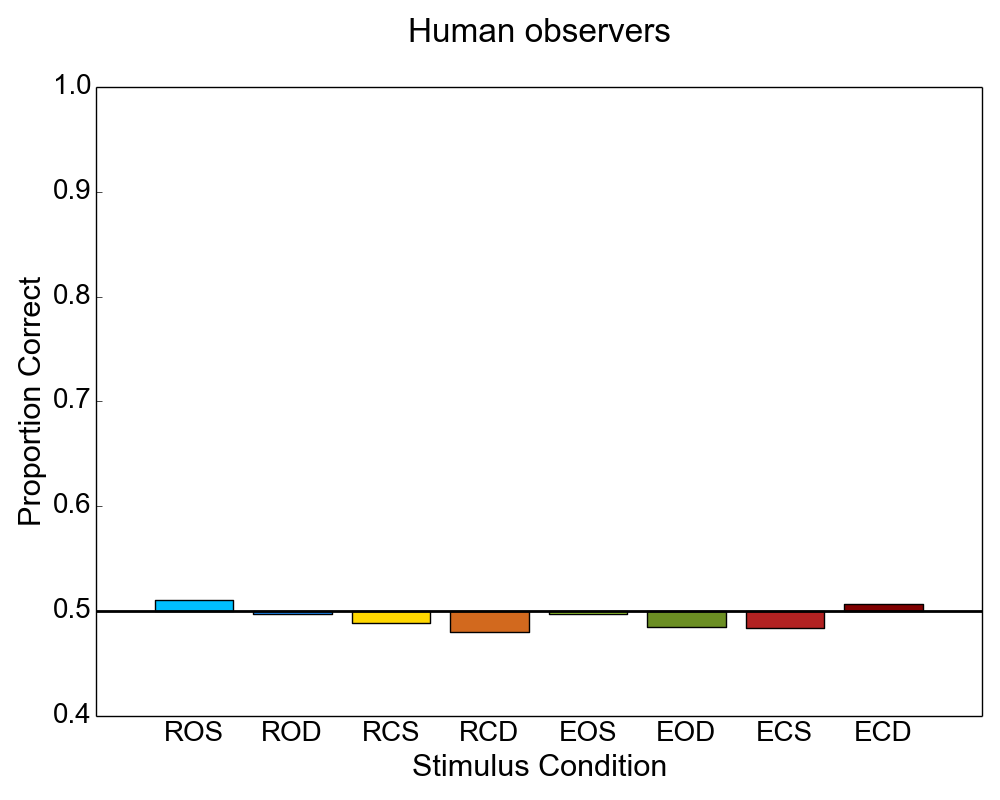
\includegraphics{Figures/FIG_detect_data_exp2.png}
\caption{Human performance in Experiment 2. The bars denote the average proportion of correct responses across observers, for the eight stimulus conditions.}
\label{fig_human_exp2}
\end{figure}

\autoref{fig_human_exp2} similarly shows the average performances for Experiment 2. It can be seen that this task proved impossible for the observers. Formal statistical testing using a t-test both on the means per condition and the overall mean returned non-significant results in all cases.


\subsection{Ideal observers: Detection}\label{subsection_results_detect_ideal}
\subsubsection{Experiment 1}
Here, we evaluate how well the ideal observers detected local density differences when performing the same 2-IFC experiment as the human observers. We obtained for each ideal observer a binary response (correct/incorrect) on each trial in the experiment, and we fitted logistic functions to these data. \autoref{fig_detect_voronoi_exp1} shows the ideal observer results for the \emph{Voronoi} metric. From the logistic fits we calculated the 75\%-thresholds; for all other metrics we will only plot the thresholds instead of the full data, to provide a clearer overview of the results.

\begin{figure}[h!]
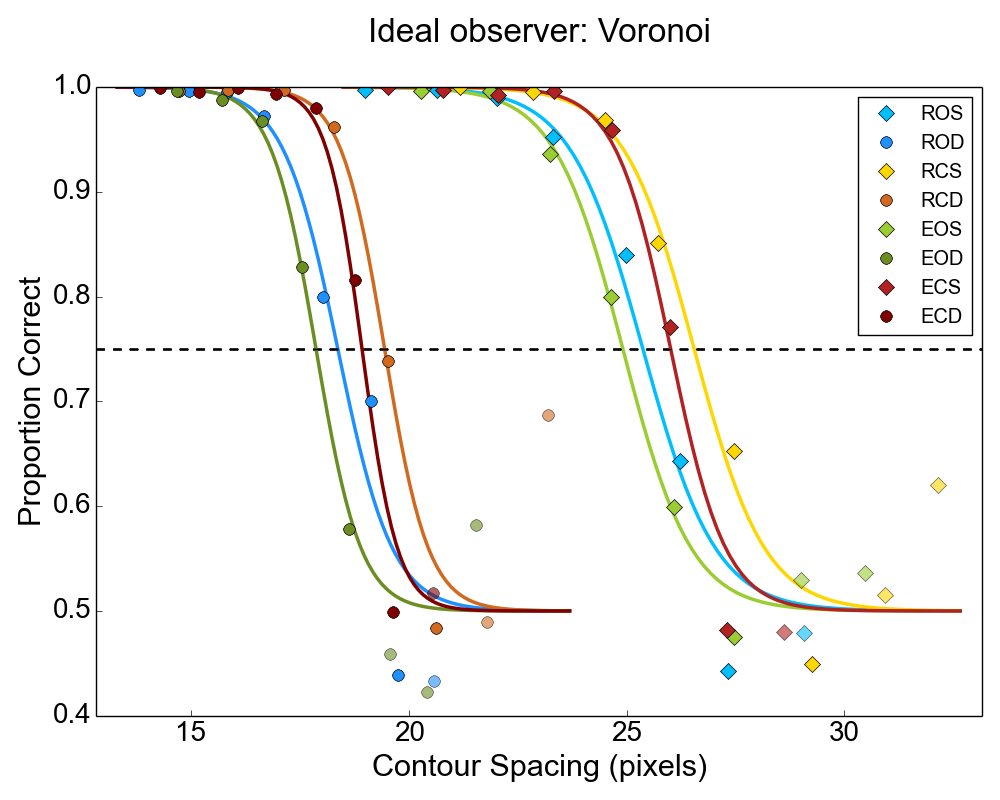
\includegraphics{Figures/FIG_detect_Voronoi_exp1.png}
\caption{Performance of the \emph{Voronoi} ideal observer on the 2-IFC task in Experiment 1. Transparent markers correspond to conditions where on average the metric considered the contour to be less dense than the background; these data points were assigned a value of 0.50 in the logistic fits. The dotted horizontal line represents the 75\%-threshold used for a comparison to the other metrics}
\label{fig_detect_voronoi_exp1}
\end{figure}

Note the qualitative similarity between the performance of the \emph{Voronoi} ideal observer (\autoref{fig_detect_voronoi_exp1}) and the performance of the human observers (\autoref{fig_human_exp1}). Performance decreased with increased spacing between contour elements. Closed contours were better detected than open contours, and randomly placed contour elements led to better performance than equidistantly placed contour elements. As with the human data, we did not run statistical tests to compare the different stimulus conditions.\\

From the families of the \emph{AvgDist} and \emph{RadCount} metrics, we here, and in the remainder of the Results section, only display those that have proven to be of particular interest. The full results can be found in the Supplementary Materials (S1). For \emph{AvgDist}, these are \emph{AvgDist-1} (nearest neighbor) and \emph{AvgDist-3}. The results of the parameter free \emph{AvgDist-n} (natural neighbors) were similar to those of \emph{Voronoi}. For \emph{RadCount}, we selected \emph{RadCount-2} (twice the minimum distance between background elements) and the parameter-free \emph{RadCountFull}.\\

In \autoref{fig_detect_series_exp1} we compare the 75\%-thresholds of the \emph{Voronoi} metric to the 75\%-thresholds of the selected \emph{AvgDist} and \emph{RadCount} metrics. The average threshold across stimulus conditions is shown as the black hexagonal marker. The statistical significance of all differences was tested two-sided, at $\alpha = 0.05$, through the resampling procedure described above. The gray triangles indicate conditions (and means across conditions) that are significantly different from the \emph{Voronoi} performance, as well as the direction of the difference. Higher thresholds indicate better performance. Note that some markers fall into the upper and lower \emph{Inv}alid categories. These markers correspond to data points where more than 10\% of the simulated 75\%-thresholds fell outside the X-axis range of \autoref{fig_detect_voronoi_exp1}.\\

It can be seen that \emph{AvgDist-1} - which only takes into account the single nearest neighbor - performs better on the Random conditions, compared to \emph{Voronoi} but tends to be worse at the Equidistant conditions. \emph{AvgDist-3} is a better cue detector than \emph{Voronoi} in all conditions. \emph{RadCountFull} results in Invalid for all Equidistant stimulus categories, indicating high detection performance regardless of contour spacing. In other words, this metric detects the regularity of contour spacings in these displays. There is also an advantage present in the Random conditions, where performance is better than \emph{Voronoi}. \emph{RadCount-2} performs significantly worse than \emph{Voronoi}.

\begin{figure}[h!t]
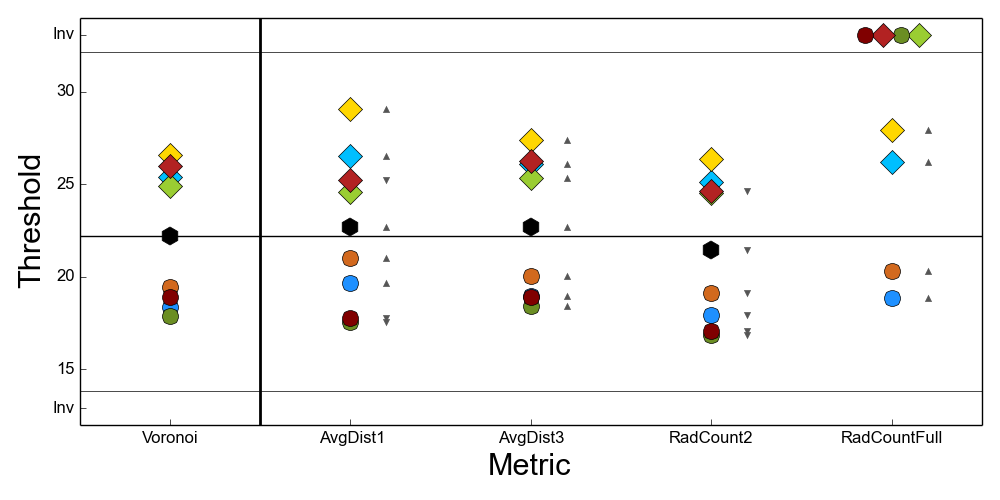
\includegraphics{Figures/FIG_detect_series_exp1.png}
\caption{Comparison of 75\%-thresholds in Experiment 1 between the \emph{Voronoi} metric and the selected \emph{AvgDist} and \emph{RadCount} metrics (colors and marker types as in \autoref{fig_human_exp1} and \autoref{fig_detect_voronoi_exp1}). The number following a metric's name corresponds to the number of nearest elements used to calculate the average distance from an element to its neighbors, or the fixed radius (in units of minimal background element distance) used, respectively. Black hexagons represent the average threshold across stimulus conditions; significant differences from \emph{Voronoi}, and their  direction, are indicated by triangular markers. The Inv (invalid) categories hold data points where the 75\%-thresholds exceed the data range.}
\label{fig_detect_series_exp1}
\end{figure}

\subsubsection{Experiment 2}

\autoref{fig_detect_series_exp2} similarly plots the ideal observer performances for Experiment 2, in its single contour spacing condition. It can be seen that whereas humans were unable to do this task, the ideal observers perform well. This is especially the case for the \emph{Voronoi} metric, the \emph{AvgDist} metrics, and the \emph{RadCountFull} metric. The fixed-radius \emph{RadCount-2} metric performs worse. In general, the Open contours are less easily detected, especially in conditions with Random element placement.

\begin{figure}[h!t]
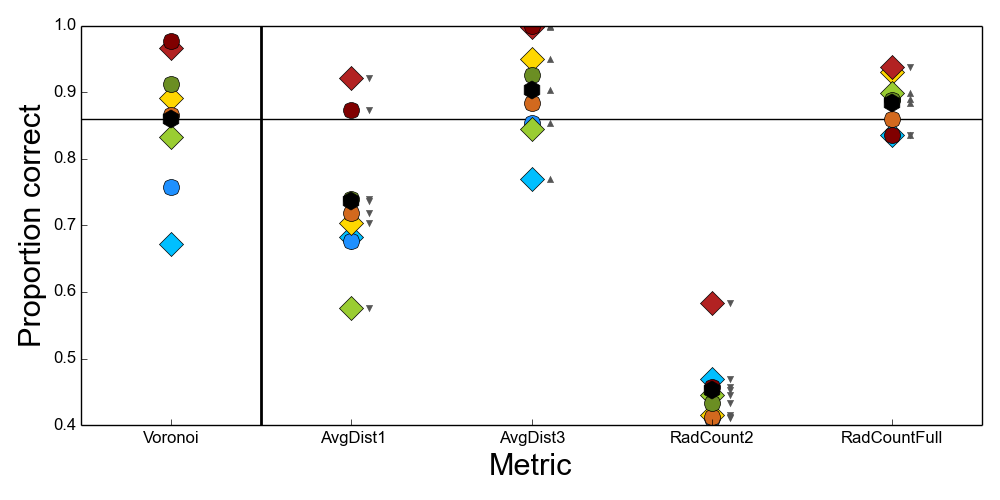
\includegraphics{Figures/FIG_detect_series_exp2.png}
\caption{Comparison of performances in Experiment 2 between the \emph{Voronoi} metric and the selected \emph{AvgDist-n} and \emph{RadCount-r} metrics. Colors and marker types correspond to \autoref{fig_human_exp1} and \autoref{fig_detect_series_exp1}.}
\label{fig_detect_series_exp2}
\end{figure}


\subsection{Ideal observers: Prediction}\label{subsection_results_predict}

\subsubsection{Experiment 1}

Here, we quantify each metric's ability to predict the 64 \emph{condition means} of the human detection data, averaged across participants. We fitted a linear curve on the eight logit-transformed data points of each display type condition, and computed the \emph{Within-Condition} fit $\overline{r}^{2}_W$ as the mean squared correlation (explained variance) within conditions. To obtain the \emph{Between-Condition} fit value, i.e. the consistency across display types, we computed the squared correlation $r^{2}_B$ across all 64 conditions means, and subtracted from this $\overline{r}^{2}_W$. \autoref{fig_predict_voronoi_exp1} illustrates our approach for the \emph{Voronoi} metric. High values of $\overline{r}^{2}_W$ indicate a good correspondence between humans and ideal observers, whereas low values of $r^{2}_B -\overline{r}^{2}_W$ indicate good generalizability across display types. Clearly, the \emph{Voronoi} metric corresponds well to human performance, confirming the qualitative similarity between \autoref{fig_human_exp1} and \autoref{fig_detect_voronoi_exp1}.

\begin{figure}[h!]
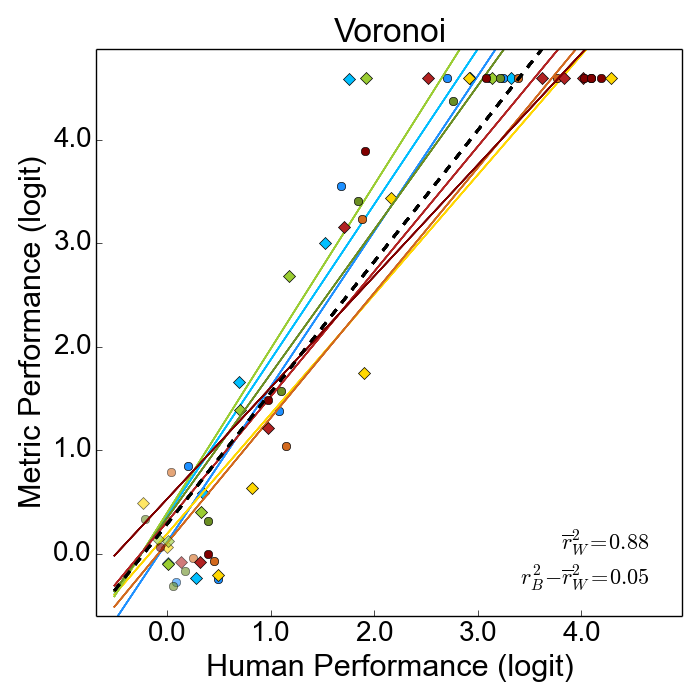
\includegraphics{Figures/FIG_predict_Voronoi_exp1.png}
\caption{Comparison between the 64 mean condition performances of human observers and the corresponding performances of the \emph{Voronoi} ideal observer. The colored lines are the condition-specific linear fits through all eight data points of each condition. The dotted black line is the linear regression line through all data points. $\overline{r}^{2}_W$ quantifies the individual condition fits, whereas $\overline{r}^{2}_W-r^{2}_B$ quantifies the variability across condition fits.}
\label{fig_predict_voronoi_exp1}
\end{figure}


\begin{figure}
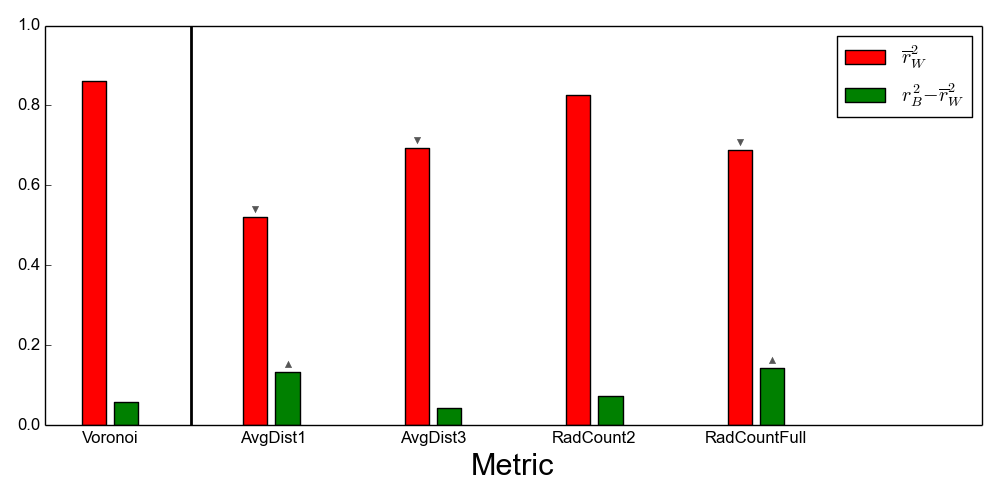
\includegraphics{Figures/FIG_predict_series_exp1.png}
\caption{Comparison of predictive validity between the \emph{Voronoi} metric and the selected \emph{AvgDist} and \emph{RadCount} metrics. $\overline{r}^{2}_W$ is the within-condition coefficient of determination, averaged across conditions; $r^{2}_B$ is the coefficient of determination across all eight stimulus conditions. High values of $\overline{r}^{2}_W$ (red bars) indicate strong within-condition correspondence between a metric and the human data. Low values of $r^{2}_B -\overline{r}^{2}_W$ (green bars) indicate a high consistency across stimulus conditions. Statistical significance is indicated through the triangular markers.}
\label{fig_predict_series_exp1}
\end{figure}

In \autoref{fig_predict_series_exp1}, we statistically compare the obtained values for the \emph{Voronoi} metric to the selected other metrics, following the same general resampling logic detailed above. None has better predictive validity of the condition means than the \emph{Voronoi} metric. Only \emph{RadCount-2} is statistically similar to \emph{Voronoi} in predicting human performance within and across stimulus conditions.

\subsubsection{Experiment 2}
We did not analyze the predictive validity of the ideal observer models for Experiment 2, since humans were unable to detect any target displays in this part of the study. The predictive validity can be expected to be very low.


\subsection{Ideal observers: Selection}\label{subsection_results_select}

\subsubsection{Experiment 1}

Predicting condition means, although possibly elucidating, is however not the main application of these local density cue metrics. Foremost, we want to evaluate how well human observers can still detect the presence of a target contour in \emph{each individual display} given the \emph{p} outputted by each metric. As explained in \autoref{subsection_methods_metrics}, a \emph{p} of 0.5 indicates equal density for contour and background elements given a specific metric, while lower or higher values of \emph{p} signal more dense or more sparse contours, respectively.\\

\autoref{fig_select_voronoi_exp1} plots the dependence of human performance on \emph{p} for the \emph{Voronoi} metric. The values \emph{p} returned by the metric are binned into six categories. The first four categories on the X-axis in \autoref{fig_select_voronoi_exp1} contain values \emph{p} corresponding to contours being more dense than the background. The fifth bin is centered around a \emph{p} of 0.5, where the metric judges contour and background to be equally dense. The last bin contains large values of \emph{p}, indicating that the contour is less dense than the background. For each bin of \emph{p}, the mean human performance on trials within that bin is displayed, separately for each stimulus condition. The marker size is proportional to the number of stimuli in each \emph{p}-bin. The black line connects their weighted means across stimulus conditions. A performance over 90\% is reached for very low values of \emph{p}, dropping to 55.7\% in the $0.35 < p < 0.65$ category where the density cue is, according to the \emph{Voronoi} metric, said to be absent. Performance drops even further to around 51.3\% for the $0.65 < p <1.0$ stimuli, where the metric judged the contour to be sparser in local density than the background elements. This is still significantly higher than the 50\% chance level (z=2.27).\\

\begin{figure}
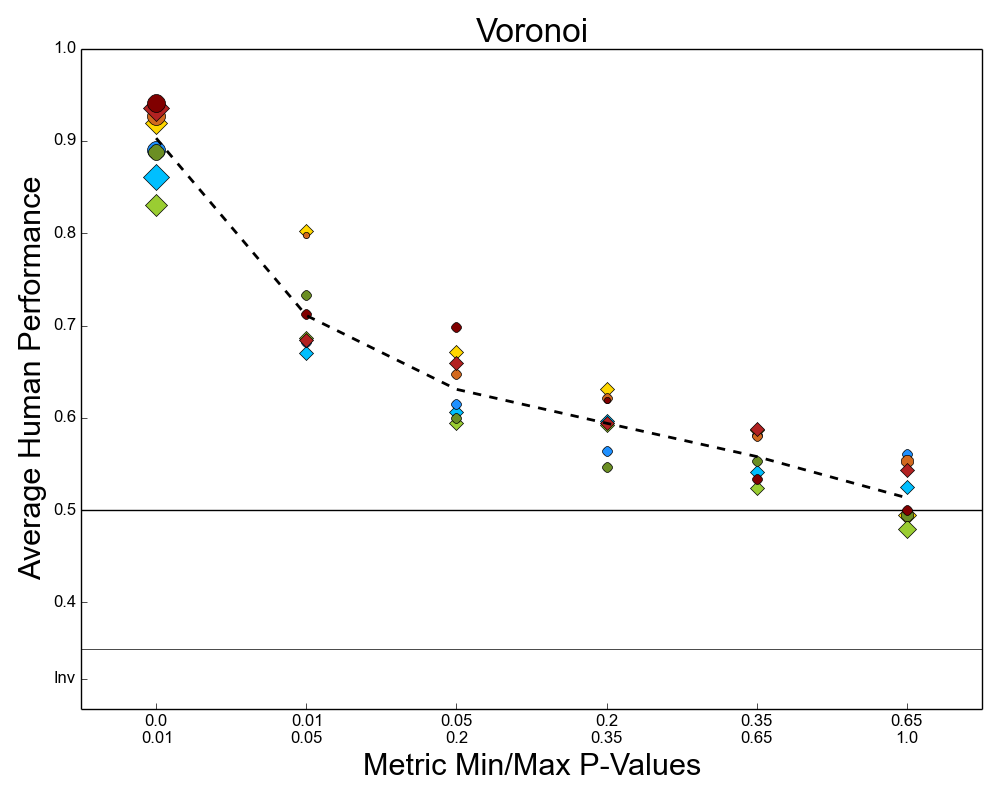
\includegraphics{Figures/FIG_select_Voronoi_exp1.png}
\caption{Average human performance on subsets of trials selected on the basis of the \emph{p}-value returned by the \emph{Voronoi} metric. Condition-specific markers as in \autoref{fig_human_exp1} and \autoref{fig_detect_voronoi_exp1}. The marker size is proportional to the number of stimuli retained in each bin of \emph{p}. The black dotted line connects their weighted means across stimulus conditions.}
\label{fig_select_voronoi_exp1}
\end{figure}

For comparison to the selected other metrics, we consider only the latter two bins of \emph{p}.

\autoref{fig_select_series_exp1_3565} shows the average human performance for trials with $0.35 < p < 0.65$ on a given metric. For these trials, the metric of interest yields (almost) no evidence for the presence of a local density cue. Human performance on trials selected according to this criterion is overall best for the \emph{Voronoi} metric, although it is statistically similar for the \emph{AvgDist-3}. Interestingly, \emph{AvgDist-1} is excellent at selecting the Random display types. \emph{RadCountFull} predictably has next to no data points in the Equidistant conditions, where it almost always detects a density cue. In the Random conditions however, it slightly outperforms \emph{Voronoi}. \emph{RadCount-2} on the other hand is a significantly worse display selection metric on all fronts.

\begin{figure}
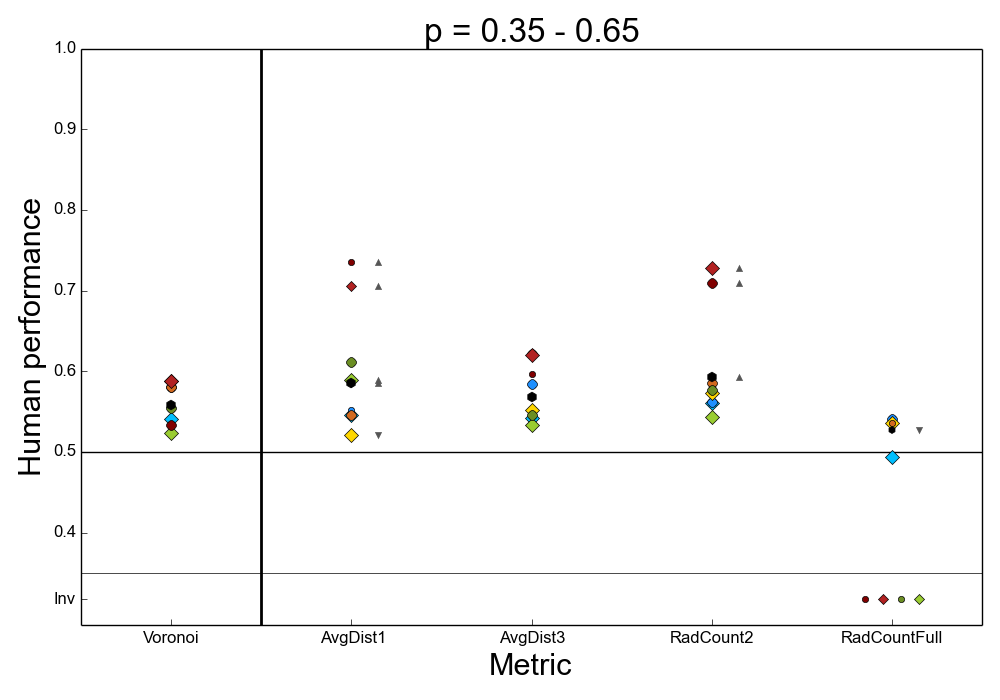
\includegraphics{Figures/FIG_select_series_exp1_3565.png}
\caption{Average human performance on a subset of trials for which the metric of interest returned a \emph{p} between 0.35 and 0.65 (i.e., almost complete absence of density cue, according to the metric).}
\label{fig_select_series_exp1_3565}
\end{figure}

\autoref{fig_select_series_exp1_651} displays the results for the category $0.65 < p < 1$, where the contour is significantly more sparse than the background. Here, only \emph{AvgDist-3} is significantly better than \emph{Voronoi}, and at a mean performance of 50.3\%, human contour detection is no longer significantly better than chance (z=0.6). The variability across stimulus conditions is low, without any apparent systematicity.\\

\begin{figure}
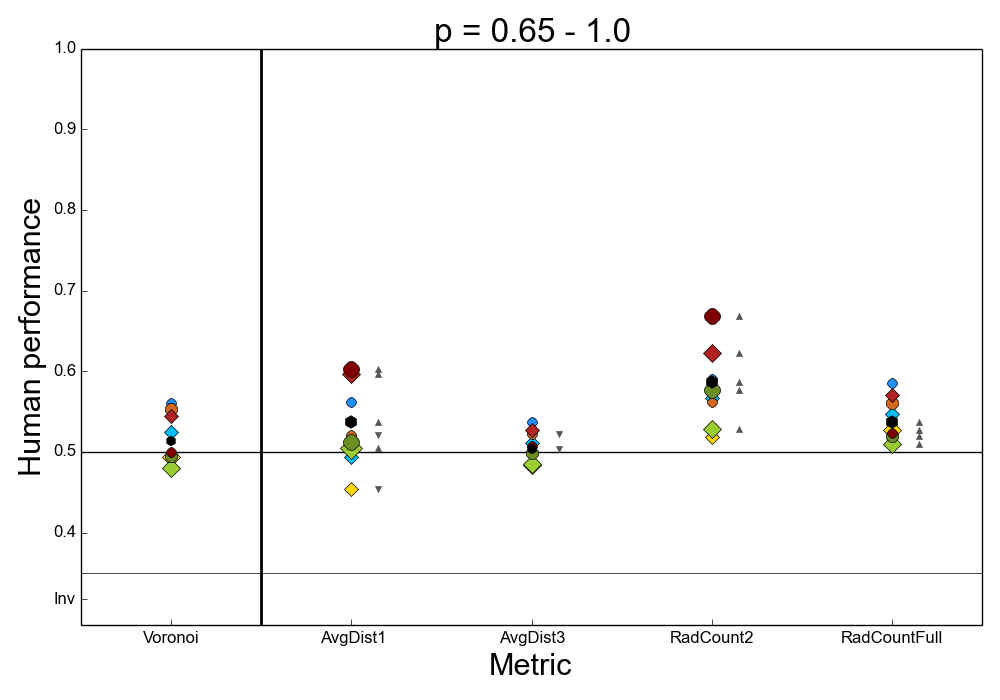
\includegraphics{Figures/FIG_select_series_exp1_651.png}
\caption{Average human performance on a subset of trials for which the metric of interest returned a \emph{p} between 0.65 and 1.0 (i.e., contour more sparse than background, according to the metric).}
\label{fig_select_series_exp1_651}
\end{figure}


\subsubsection{Experiment 2}
We have not analyzed the stimulus selection performance of the ideal observer models for Experiment 2. Evaluating how different stimulus selection criteria relate to human performance would be purposeless, since human performance was at chance in Experiment 2.


%%
% Discussion
%%
\section{Discussion}\label{section_discussion}

\subsection{Human performance}\label{subsection_discussion_human}
The analysis of human performance in Experiment 1 shows that sensitivity to local density cues depends on the specific type of grouping display. Closed contours are more salient than Open contours, a result in line with \citeA{Pettet98}. Note, however, that the Closed contours are longer, and have more contour elements and more neighboring pairs of contour elements \cite<see also>{Tversky04} than the Open contours. Random placement of contour elements, surprisingly, improves detection of density cues compared to Equidistant placement of contour elements. To understand this, consider how Equidistant element placement puts all neighboring contour elements at a regular intermediate distance from one another, whereas Random placement leaves the possibility of closer clustering for some pairs of elements. This suggests that the regularity of contour element placement is only a weak cue to human observers, compared to the stronger proximity cue created by the closer local pairings of neighboring contour elements.\\

Importantly, Experiment 2 shows that human observers are unable to detect contours that are more sparsely distributed than the background they are embedded in, even when explicitly instructed to detect such contours through positional cues. This result is in line with earlier observations by Kov{\'a}cs and colleagues \citeyear{Kovacs99, Kovacs00}.

\subsection{Ideal observer performance}\label{subsection_discussion_ideal}

Many of the ideal observer models tested perform well, both in detecting density cues and in predicting human performance. It should also be noted that in most cases, the results generalized across the different stimulus conditions, confirming these metrics as excellent general tools during stimulus construction. What the single `best' metric is however, strongly depends on the aims of the researcher. \\

\underline{Physical cue detection.} 
To optimally detect purely the physical presence of a contour in a display, \emph{RadCountFull} is at first sight the best option. Not only does this metric detect all Equidistant target displays, it is also a top performer for the Random conditions. However, one must consider that rejecting Equidistant conditions based on its regularity cue is fairly trivial, when that regularity cue was part of the stimulus design. For the Random conditions on the other hand, the much less computationally intensive \emph{AvgDist-3} metric performs comparably, at least for Experiment 1.

In addition, it is interesting to note that the \emph{AvgDist-1} metric, i.e. the distance to the single nearest neighbor, performs well on all Random conditions. The qualitative resemblance to the human tendency to perform better on these conditions, for the speculative reasons outlined above, is striking.\\

\underline{Human cue detection.} 
If one is prepared to consider human sensitivity to density cues in the stimulus construction process, it is obvious that using sparser contour spacings compared to the background spacing will minimize a subject's ability to detect a contour based on positional cues - even though most ideal observer models have no problem with this task. One caveat should be made, however. We measured a single level of contour element spacing for Experiment 2; if one would further increase the sparseness of the contour, background elements could gradually be placed in-between the contour elements, at least when using GERT's default routines for element placement. Naturally, this will be disruptive to the actual grouping process under study. \emph{AvgDist-3} is a particularly useful metric when moderately sparse contours are used, with human performance consistently around chance in the $0.65<p<1$ stimulus selection category for all display types.

The superior ability of \emph{RadCountFull} to detect regularity in contour element placement becomes even more irrelevant when human sensitivity is taken into account, since human observers are hardly sensitive to the regularity cue. This has a large bearing on \emph{RadCountFull}'s performance in \autoref{fig_predict_series_exp1}, where the overall correspondence to human condition means is shown to be comparatively poor.\\

To evaluate the presence of a minimally detectable cue that does \emph{not} involve the deliberate use of sparser contours, we considered the $0.35<p<0.65$ category during stimulus selection. Here, \emph{Voronoi}, \emph{RadCountFull} (on Random conditions), and \emph{AvgDist-3} performed similarly well, although \textit{Voronoi} displayed less spread across display type conditions. With an average human performance of 55.7\%, the cue is nearly eliminated at this level of \emph{p}. At this point, we would again like to bring into attention the fact that participants in this study performed an explicit local density detection task, with orientation-less circular Gabors. We consider this a liberal estimate of the degree to which subjects would benefit from a density cue in for instance a collinearity detection task, where local density is not the cue of interest, and where randomness (background) and jitter (contour) to the Gabor orientations constitutes a disruption to perceptual grouping \cite<e.g.,>{Field93}.\\

\subsection{Improved metrics}\label{subsection_discussion_improved}

Still, even with the most stringent $0.35<p<0.65$ stimulus selection criterion and the most sensitive local density metric, human observers perform above chance in Experiment 1 (\autoref{fig_select_series_exp1_3565}). This does leave room for the development of better local density metrics for physical cue detection, for predicting condition means of human performance, and for prediction of contour detection on individual displays. The current dataset and accompanying analysis scripts have been made public to allow the standardized evaluation of new metrics (URL: \href{https://github.com/mpjdem/densitycue}{https://github.com/mpjdem/densitycue}).\\

\begin{figure}
<<<<<<< HEAD
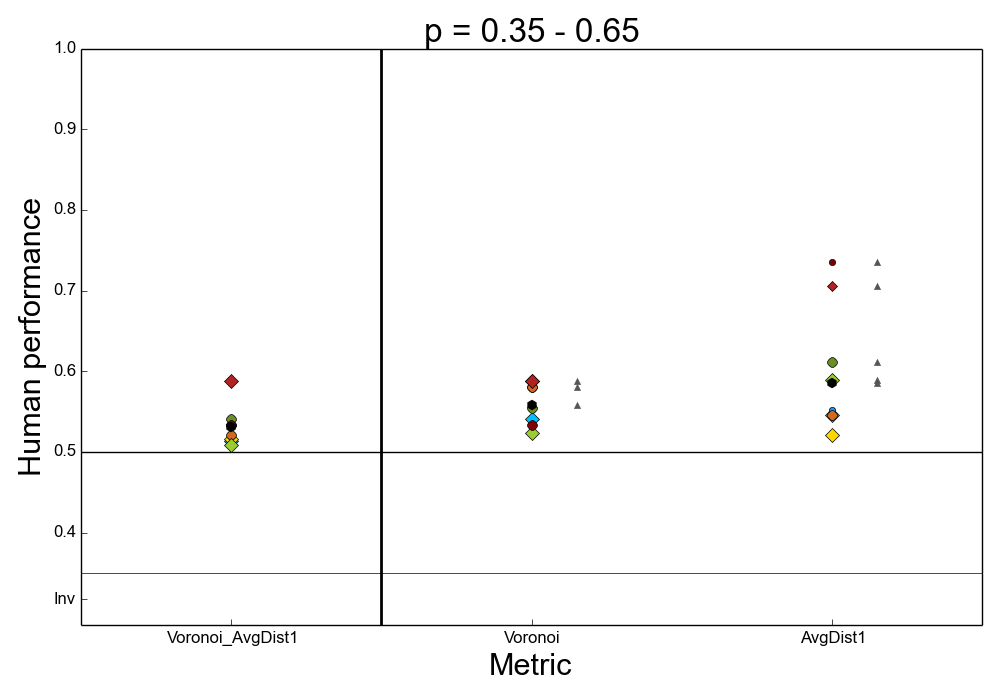
\includegraphics{Figures/FIG_select_combined_exp1_3565.png}
=======
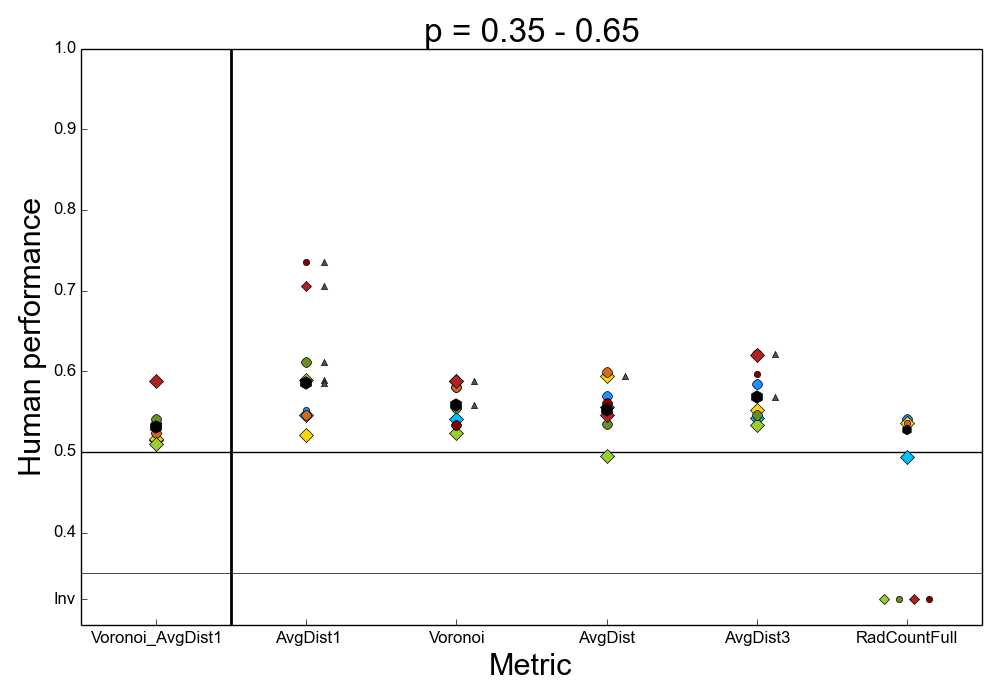
\includegraphics{Figures/FIG_select_series_Voronoi_AvgDist1_3565}
>>>>>>> 0c9ff40... misnamed figure
\caption{Comparison between the \emph{Voronoi} and \emph{AvgDist-1} metrics and their combination for the average human performance on a subset of trials for which the metric of interest returned a \emph{p} between 0.35 and 0.65 (i.e., almost complete absence of density cue, according to the metrics).}
\label{fig_select_combined_exp1_3565}
\end{figure}

One valuable approach would be to combine multiple density metrics. For instance, we have speculated that humans are sensitive to Random conditions because of local clustering of contour elements, and have noted that the \emph{AvgDist-1} metric is more sensitive to Random conditions than other metrics are. Indeed, combining \emph{AvgDist-1} with \emph{Voronoi} such that the lowest value \emph{p} of both tests is retained, leads to a significantly better metric for stimulus construction within the $0.35<p<0.65$ selection bin, as shown in \autoref{fig_select_combined_exp1_3565}, with an average human performance of 53\%. Only the ECS display type retains a somewhat higher human performance. An alternative approach is to define new metrics based on other geometric relations between the display elements. One avenue could be the use of genetic algorithms that have the potential to find the specific combination of spatial relations in the display that best explains human performance on the task.

\subsection{Alternative approaches}\label{subsection_discussion_alternative}

The density metric D \cite{Kovacs93,Kovacs94,Kovacs99,Kovacs00}, discussed in the Introduction, is largely comparable to the \emph{AvgDist} family of metrics implemented in GERT. However, because D does not provide individual local density estimates for each element in the display, it cannot be evaluated using the procedures of the current manuscript. In the Supplementary Materials (S2), we have nonetheless computed D for all trials run in Experiments 1 and 2, and have plotted human performance against D. It can be seen that the D=0.85 criterion often used in this literature is indeed appropriate for reducing contour detection performance to chance, when using unoriented elements.\\

In addition, we have computed a denstiy cue metric based on the average luminance difference in contour and background regions of the stimulus image, following low-pass filtering. This could be regarded as a more generic alternative to the explicit grouping by proximity of element positions. However, as the Supplementary Materials (S3) demonstrate, such luminance metric does not allow a display selection comparable in reliability to the results obtained above.\\

\subsection{Recommendations}\label{subsection_discussion_recommendations}

(1) When using the best-performing metrics of the current study for the elimination of density cues in grouping displays, the results obtained will be largely independent of the stimulus type used, at least with regard to contour closure, overall display density, and regularity of contour element placement. The most notable exception to this is that the \emph{RadCountFull} metric will always reject stimuli with Equidistant contour element placement.

(2) For elimination of a local density cue to the presence of a contour that can either be more sparse or more dense than the surrounding background elements, use the fast parameter-free \emph{Voronoi} metric with a \emph{p} criterion between 0.35 and 0.65 to achieve near-chance potential detection of a density cue. Further improvement is attained by combining this metric with the \emph{AvgDist-1} metric.

(3) To attain even lower human density cue detection performance, select moderately sparser contours, compared to the background element density. Chance performance can be expected when using the \emph{AvgDist-3} metric, with a selection criterion of $p > 0.65$.

(4) The confounding effect of any remaining difference in local density between contour and background can be further reduced by adopting the logic of \citeA{Geisler01}. These authors embedded a contour in target-absent as well as target-present displays, but removed the collinearity cue of interest in the former by randomly orienting the contour elements. Target-absent displays then contain the same positional information as target-present displays. This ensures that a local density cue by itself can never be informative to the task - although its interaction with collinearity might still be informative.


%%
% Conclusion
%%
\section{Conclusions}
We have validated the general stimulus selection approach of the Grouping Elements Rendering Toolbox. The values \emph{p} yielded by its local density metrics perform well in many cases, both in physical cue detection and in the prediction of human performance. Moreover, their validity generalizes across a range of display types.

With regard to human processes of grouping by proximity, we especially note that contours with a more sparse element density than their surrounding distractor elements are nearly undetectable, and that regularity in contour element spacing is a weak cue compared to the local high-proximity clusters of randomly placed contour elements.


%%
% Acknowledgments
%%
\section{Acknowledgments}
BM and MD are post-doctoral fellows of the Research Foundation-Flanders (FWO). This work was supported by a Methusalem grant by the Flemish Government (METH/08/02) awarded to JW. We would like to thank Eveline Smolders for collecting the empirical data.


%%
% References
%%

\bibliography{manuscript.bib}{}
\bibliographystyle{apacite}


%%
% Appendices
%%


%%
% The End
%%
\end{document}
